\documentclass[letterpaper]{article}
\usepackage[submission]{aaai2027}
\usepackage[hyphens]{url}
\usepackage{graphicx}
\urlstyle{rm}
\def\UrlFont{\rm}
\usepackage{natbib}
\usepackage{caption}
\frenchspacing
\usepackage{booktabs}
\usepackage{amsmath}
\usepackage{amsfonts}
\usepackage{amssymb}
\usepackage{multirow}

\allowdisplaybreaks
\setcounter{secnumdepth}{2}
\renewcommand{\thetable}{S\arabic{table}}
\renewcommand{\thefigure}{S\arabic{figure}}

\title{Technical Appendix for\\
SPRiF: Spectral Projective Reset Integrate-and-Fire Neuron}
\author{Anonymous Submission}
\affiliations{}
\date{}

\begin{document}

\maketitle

\section{Appendix Guide and Evidence Map}
\label{supp:sec:guide}

This technical appendix provides reproducibility details for the five benchmark results, exact definitions of the mechanism variants and SI-DMS intervention, the formal SPRiF update equations, and the associated protocols for analyzing the dynamics.

\paragraph{Reporting conventions.}
The slow spectral state has three coordinates, the fast discharge state has two, and each timestep follows $I_t\to\mathbf{x}_t\to\widetilde{\mathbf{u}}_t\to v_t\to z_t\to\mathbf{u}_t$. The direct reset at the current timestep acts only on the fast discharge state, with $\Delta\mathbf{x}_t^{\mathrm{reset}}=\mathbf{0}$. In recurrent layers, spikes can affect the next update of the slow state through the ordinary $W_{\mathrm{rec}}\mathbf{z}_t$ input pathway.

Throughout the appendix, \emph{slow spectral state}, \emph{fast discharge state}, and \emph{projective reset} follow the definitions in the main text. Benchmark SPRiF entries report mean$\pm$standard deviation over five seeds, SI-DMS entries summarize three seeds, and published comparator entries provide descriptive context from prior studies.

\paragraph{Evidence map.}
The sections below provide the supporting details for specific elements of the main text:
\begin{itemize}
\item Table~1 in the main text is expanded by the dataset encodings, architectures, optimization settings, and reporting rules in Sections~\ref{supp:sec:protocols}--\ref{supp:sec:reporting}; the SPRiF entries are estimates over five seeds, and published comparator entries provide descriptive context.
\item Table~2 in the main text is expanded by the variant definitions in Section~\ref{supp:sec:variant-definitions}: $\omega=0$, the merged slow/fast state, and $\lambda=0$.
\item The SI-DMS results are expanded by the recurrent task construction, definition of paired loss, sweep over intervention fractions, coverage across delays and $K$, and implementation checks in Sections~\ref{supp:sec:sidms-protocol}--\ref{supp:sec:sidms-integrity}. Training uses $K\in\{0,1,2,4,8\}$ at a fixed 15\% intervention fraction; evaluation extends to $K\in\{16,32,40\}$ and fractions from 5\% to 50\%.
\item The S-MNIST loss landscape diagnostic in Section~\ref{supp:sec:loss-landscape} analyzes the local sensitivity of one saved checkpoint per model, using one training seed and one pair of random directions.
\item The mechanism and temporal kernel figures are expanded by the reset identities and impulse and spectral protocols in Sections~\ref{supp:sec:dynamics}--\ref{supp:sec:analysis-protocols}.
\item Section~\ref{supp:sec:perturbation-diagnostic} reports the responses of saved checkpoints under fixed feature perturbations.
\end{itemize}

\begin{table*}[tbp]
\centering
\small
\setlength{\tabcolsep}{3pt}
\begin{tabular}{lccccc}
\toprule
Item & S-MNIST & PS-MNIST & QTDB & GSC & SHD \\
\midrule
Input dimension & 1 & 1 & 4 & 120 & 700 \\
Output dimension & 10 & 10 & 6 & 12 & 20 \\
Layer & 1--64--210--10 & 1--64--210--10 & 4--31--6 & 120--300--12 & 700--64--20 \\
Epochs & 150 & 150 & 250 & 150 & 100 \\
Optimizer & Adam & Adam & Adam & Adam & Adam \\
Batch size & 512 & 512 & 128 & 128 & 100 \\
Learning rate & $10^{-2}$ & $10^{-2}$ & $10^{-2}$ & $5\times10^{-3}$ & $10^{-2}$ \\
Loss & CE & CE & CE & CE & CE \\
LR decay & 0.1 / 50 ep & 0.1 / 50 ep & 0.65 / 100 ep & 0.5 / 30 ep & 0.5 / 20 ep \\
LR decay type & StepLR & StepLR & StepLR & StepLR & StepLR \\
Threshold & 1.0 & 1.0 & 0.6 & 0.8 & 1.0 \\
$\tau_\alpha$ (steps) & [2, 60] & [2, 60] & [20, 120] & [10, 80] & [10, 80] \\
$\tau_\rho$ (steps) & [2, 40] & [2, 40] & [4, 30] & [4, 30] & [4, 30] \\
$\tau_\eta$ (steps) & [0.8, 10] & [0.8, 10] & [0.8, 8] & [0.8, 8] & [0.8, 8] \\
$\omega$ ($\times\pi$) & [0.04, 0.50] & [0.04, 0.50] & [0.02, 0.20] & [0.04, 0.40] & [0.04, 0.40] \\
\bottomrule
\end{tabular}
\caption{Architecture and optimization settings for the SPRiF benchmark entries. Architecture entries list input, recurrent hidden, and output widths; S-MNIST and PS-MNIST use two recurrent hidden layers. LR decay denotes the StepLR multiplier and interval, and CE denotes cross-entropy.}
\label{tab:supp_arch}
\end{table*}

\section{Experimental Protocols and Reporting}
\label{supp:sec:protocols}

The five benchmark entries use inputs and readouts standard for each task. S-MNIST and PS-MNIST use MNIST~\cite{lecun1998gradient} tensors read as pixel sequences of 784 steps; PS-MNIST applies a random pixel permutation generated from the seed and fixed within the run.

QTDB uses the public QT Database~\cite{laguna1997database} and adopts the preprocessing protocol from \emph{Accurate and Efficient Time-Domain Classification with Adaptive Spiking Recurrent Neural Networks}~\cite{asrnn}. Increasing and decreasing level-crossing events convert two normalized ECG channels into four input event streams, and a classifier predicts six waveform classes at each timestep. The released QTDB utilities expose \texttt{convert\_seq}, which applies Savitzky--Golay smoothing followed by thresholded positive and negative events from first differences, and \texttt{convert\_dataset\_wtime}, which unpacks the encoded \texttt{x}, \texttt{y}, and \texttt{t} arrays and derives intervals between timesteps. Training consumes the resulting \texttt{QTDB\_train.mat} and \texttt{QTDB\_test.mat} files.

GSC uses one-second utterances from Google Speech Commands~\cite{warden2018speech}, represented as mel features with 40 bins and first- and second-order deltas stacked over 101 frames, followed by temporal mean pooling over hidden spikes. SHD uses cochlea event sequences with 700 channels from the Spiking Heidelberg Digits dataset~\cite{cramer2022heidelberg}, with recurrent hidden processing and accumulated readout evidence after warm-up.

The benchmark set covers complementary temporal regimes. S-MNIST tests retention over a long serialized image, PS-MNIST removes spatial locality through a fixed permutation, QTDB requires dense classification of physiological signals at each timestep, GSC tests dense acoustic features over an utterance, and SHD tests sparse input represented as events. Together they span sequence structure, modality, and readout conventions. The comparisons with published results provide context across protocols that differ by task.

\subsection{Architectures and Optimization}
\label{supp:sec:architectures}

Table~\ref{tab:supp_arch} reports the network and optimization settings for each task in the submitted SPRiF runs. Ranges for $\omega$ are expressed as multiples of $\pi$.

For S-MNIST and PS-MNIST, truncated BPTT uses a chunk length of 262 steps. The GSC network uses temporal mean pooling over hidden spikes before the linear classifier. The QTDB network optimizes the sequence loss at each timestep. SHD accumulates readout evidence after the warm-up period. All models use the multi-Gaussian surrogate gradient described in Section~\ref{supp:sec:surrogate}.

During development, candidate settings were explored within the following envelopes: learning rate $[4\times10^{-5},5\times10^{-2}]$, threshold $[0.3,1.5]$, $\tau_\alpha\in[1,140]$ steps, $\tau_\rho\in[1,80]$ steps, $\tau_\eta\in[0.2,20]$ steps, and $\omega\in[0.05,2.0]$ radians. Candidate settings were sampled within these bounds, and the final settings for each task were fixed across the five reported seeds. Table~\ref{tab:supp_arch} reports the final settings and initialization intervals used for the submitted runs.

\subsection{Seeds, Model Selection, and Reporting}
\label{supp:sec:reporting}

All five benchmarks use the seed set $\{0,1,2,42,1111\}$. Table~1 reports the mean and standard deviation of those selected accuracies over five independently seeded runs. Within a task, all runs use the same preprocessing, data splits, and architecture settings in Table~\ref{tab:supp_arch}; only the seeded training realization changes. Published comparator entries provide context under their original protocols. SI-DMS is a separate recurrent mechanism experiment using seeds $\{1,2,3\}$. For its summary statistics, each seed is first averaged over the five evaluation delays; the reported mean and sample standard deviation are then computed over the three resulting values.

The released benchmark utilities seed Python's \texttt{random} module, NumPy, PyTorch on CPU, and all visible CUDA devices; they also disable cuDNN benchmarking. SI-DMS uses the same seed to initialize these four sources of randomness. It also constructs a separate \texttt{torch.Generator} for each condition so that compared models receive identical cue tensors and intervention masks within each seed/delay/$K$/fraction condition. These controls reproduce the principal random choices. Different hardware and software stacks may not produce bitwise identical results.

\subsection{Evaluation Metrics and Uncertainty}
\label{supp:sec:metrics}

Accuracy is the primary metric because every benchmark is a classification task with one label and the cited comparator literature reports accuracy. S-MNIST, PS-MNIST, GSC, and SHD use the fraction of correctly classified sequences; QTDB uses the fraction of correctly classified labeled timesteps under its readout at each timestep. SI-DMS uses match/non-match accuracy for each sequence together with the paired intervention loss in Eq.~\eqref{eq:supp_sidms_drop}. Accuracy measures task capability, while the paired loss separates the additional degradation caused by controlled spike interventions from differences in clean accuracy.

For $S$ independent training seeds with accuracies $a_s$, we report
\begin{equation}
\bar a=\frac{1}{S}\sum_{s=1}^{S}a_s,\qquad
s_a=\sqrt{\frac{1}{S-1}\sum_{s=1}^{S}(a_s-\bar a)^2}.
\label{eq:supp_seed_summary}
\end{equation}
Using the displayed means and standard deviations, the SPRiF entries over five seeds in the main benchmark table approximately correspond to the following two-sided 95\% $t$ intervals for the seed mean: S-MNIST $[99.21,99.35]$, PS-MNIST $[95.69,96.03]$, QTDB $[87.98,88.88]$, GSC $[94.17,94.93]$, and SHD $[90.95,92.09]$ percent. These intervals quantify variation among the submitted SPRiF runs. Published comparator values use different seeds, data processing, architectures, and optimization protocols and generally do not provide results for individual seeds. The intervals therefore describe SPRiF variability, while comparisons with published results remain descriptive.

\FloatBarrier

\subsection{Compute Environment}
\label{supp:sec:compute}

Experiments were run on one NVIDIA GeForce RTX 2080 Ti GPU with 11~GB of memory and 12 vCPUs on an Intel Xeon Platinum 8255C CPU at 2.50~GHz. The software environment used Ubuntu 22.04, Python 3.12, PyTorch 2.3.0, and CUDA 12.1. Training times range from minutes for QTDB to several hours for PS-MNIST and GSC, depending on sequence length and network width. The experiments used neither distributed training nor specialized neuromorphic hardware.

\subsection{S-MNIST Loss Landscape Diagnostic}
\label{supp:sec:loss-landscape}

We probe local parameter sensitivity around trained S-MNIST solutions using a visualization on a random two-dimensional plane, inspired by loss landscapes with filter normalization~\cite{li2018visualizing}. The SPRiF and LIF models use the same two recurrent layer widths, $[64,210]$, temporal mean readout, normalized S-MNIST inputs with 784 steps, optimizer, learning rate schedule, and seed. The checkpoint metadata record test accuracies of 98.88\% for SPRiF and 95.19\% for LIF. These values describe the analyzed checkpoints from one seed, while the main benchmark reports summaries over five seeds.

For each checkpoint $\boldsymbol{\theta}^{\star}$, we generate two Gaussian random directions $\mathbf{d}_1$ and $\mathbf{d}_2$ using seeds 123 and 124. For every multidimensional parameter tensor $W$, its corresponding direction tensor $D$ is rescaled as $D\leftarrow D\lVert W\rVert_F/(\lVert D\rVert_F+10^{-10})$; one-dimensional parameters, including biases and neuron-wise dynamics parameters, are held fixed. We then evaluate
\begin{equation}
\mathcal{L}(a,b)=\mathcal{L}\!\left(\boldsymbol{\theta}^{\star}+a\mathbf{d}_1+b\mathbf{d}_2\right),
\qquad (a,b)\in[-1,1]^2,
\label{eq:supp_loss_landscape}
\end{equation}
on a $25\times25$ grid. Cross-entropy is estimated on the first four non-shuffled test mini-batches (2,048 images), with the 784-step sequence processed in chunks of 262 steps and the chunk-level logits averaged. Both models use the same coordinate range, grid resolution, and evaluation samples; the directions are normalized separately using each model's checkpoint tensors.

Figure~\ref{fig:supp_loss_landscape} shows a broader region of low loss for the analyzed SPRiF checkpoint. At the unperturbed center, the estimated cross-entropy is 0.0575 for SPRiF and 0.2098 for LIF. Over the 625 sampled coordinates, the SPRiF slice has lower loss at 85.1\% of points, with mean losses of 10.69 versus 15.78 and maxima of 36.46 versus 50.85. Under these perturbations matched by norm, this SPRiF solution is less sensitive along the sampled plane. The result is interpreted as a local sensitivity diagnostic for one checkpoint and one direction pair.

\begin{figure*}[tbp]
\centering
\includegraphics[width=0.94\textwidth]{figures/loss_landscape_smnist.png}
\caption{S-MNIST loss landscape diagnostic for SPRiF (top row) and LIF (bottom row). The 2D contours and 3D surfaces show cross-entropy over the same $25\times25$ grid of perturbation coordinates, with a shared logarithmic color scale and common vertical range. Each model uses random directions normalized by its checkpoint tensors, while evaluation samples and grid coordinates are matched.}
\label{fig:supp_loss_landscape}
\end{figure*}


\section{Mechanism Variants and SI-DMS Evaluation}
\label{supp:sec:mechanism-sidms}

\subsection{Mechanism Variant Definitions}
\label{supp:sec:variant-definitions}

Table~2 in the main text reports the ablation outcomes. Table~\ref{tab:supp_variant_defs} defines the exact model modification represented by each column.

\begin{table*}[tbp]
\centering
\small
\setlength{\tabcolsep}{4pt}
\begin{tabular}{p{0.17\textwidth}p{0.40\textwidth}p{0.33\textwidth}}
\toprule
Variant & Change relative to full SPRiF & Interpretation \\
\midrule
$\omega=0$ & Removes rotational coupling while retaining the real decay path and slow--fast state separation. & Tests spectral rotation while preserving state separation. \\
\midrule
Merged & Collapses the slow spectral state and fast discharge state into one three-dimensional state whose first coordinate is both membrane and reset target. & Tests the combined effect of collapsing memory and discharge and reducing total state dimensionality. \\
\midrule
$\lambda=0$ & Fixes the reset direction to $[1,0]^\top$, so reset subtracts only from the membrane coordinate. & Tests learned projective reset against scalar reset while preserving slow--fast separation. \\
\bottomrule
\end{tabular}
\caption{Mechanism variants corresponding to the ablation table in the main text.}
\label{tab:supp_variant_defs}
\end{table*}

Full SPRiF, $\omega=0$, and $\lambda=0$ each retain three coordinates in the slow state and two in the fast state, for five local state values per neuron. The merged variant uses a single state with three coordinates. Its result therefore reflects the combined effects of merging the states and reducing local state capacity.

\subsection{SI-DMS Protocol}
\label{supp:sec:sidms-protocol}

The Spike-Intervention Delayed Match-to-Sample (SI-DMS) task tests whether a recurrent network retains a cue through a delay while selected hidden units are forced to emit actual spikes. SI-DMS is a programmatically generated mechanism task: cue identities, Poisson spike realizations, delays, labels, and intervention masks are generated from the recorded seeds and condition settings. Table~\ref{tab:supp_sidms} gives the protocol and the controls shared across models.

\begin{table*}[tbp]
\centering
\small
\setlength{\tabcolsep}{4pt}
\begin{tabular}{p{0.20\textwidth}p{0.72\textwidth}}
\toprule
Item & Setting \\
\midrule
Input channels & 30 total: 10 left-cue channels, 10 right-cue channels, and 10 noise channels, encoded as Poisson spike trains. \\
\midrule
Pre-period & 50 ms baseline period with noise channels active. \\
\midrule
First and second cues & 100 ms each; each cue is left or right. \\
\midrule
Delay (train) & Drawn from $\{200,400,800,1600\}$ ms. \\
\midrule
Delay (eval) & Drawn from $\{200,400,800,1600,2500\}$ ms. \\
\midrule
Target & Binary match/non-match label depending on whether the two cues are identical. \\
\midrule
Intervention & At $K$ random delay timesteps, selected membrane coordinates are placed above threshold before spike computation; each resulting spike follows the model's ordinary reset rule and recurrent pathway. \\
\midrule
Intervention fraction (train) & 15\% of the 64 hidden units at each intervention timestep. \\
\midrule
Intervention fraction (eval) & $\{5,10,15,20,30,50\}\%$; the figure and table in the main text use the 15\% slice applied during training. \\
\midrule
$K$ (train) & $\{0,1,2,4,8\}$. \\
\midrule
$K$ (eval) & $\{0,1,2,4,8,16,32,40\}$; $K\in\{16,32,40\}$ are unseen during training. \\
\midrule
Shared controls & Within each seed/delay/$K$/fraction condition, models use matched batches, intervention masks, and evaluation probes. \\
\midrule
Hidden units & 64. \\
\midrule
Architecture & One recurrent spiking hidden layer followed by a two-class non-spiking leaky readout. Previous hidden spikes enter the next hidden update through a learned $64\times64$ recurrent weight matrix. \\
\midrule
Optimization & 3,000 training steps; batch size 256; Adam with learning rate $3\times10^{-3}$; gradient clipping at 1.0. \\
\midrule
Rate regularization & Natural firing rate target 0.10 with weight 0.05; intervention locations are excluded from the term for natural firing rate. \\
\midrule
SPRiF variants & \texttt{sprif\_full}, \texttt{sprif\_lambda0}, and \texttt{sprif\_merged}. \\
\midrule
Baselines & LIF, ASRNN, and BRF with the same recurrent hidden width, optimizer, batch structure, and intervention masks. \\
\bottomrule
\end{tabular}
\caption{SI-DMS task construction, controlled intervention, and controls shared across models.}
\label{tab:supp_sidms}
\end{table*}

For reproducibility of the paired replay in the main text, we use the full SPRiF checkpoint trained with seed 1 and deterministic batch seed 0 at delay 1600 ms. Clean ($K=0$) and stressed ($K=8$, nominal 15\% intervention; 10 of 64 hidden units per event) conditions receive the exact same A--A input tensor. The two A cues share stimulus identity but are independently sampled realizations of that identity. All 80 selected unit--timestep pairs in the stressed condition produce forced spikes (80/80 forced hits). Both examples have match labels and are correctly predicted as matches, and each window for the second cue contains 203 natural spikes in the hidden layer across all 64 units. The raster uses one shared set of ten units, selected jointly after excluding units naturally active in more than 40\% of delay steps. This pair illustrates the intervention protocol.

\subsection{Condition Grids}
\label{supp:sec:sidms-grids}

The result set covers six models, three seeds, five delays, eight intervention counts, and six nonzero intervention fractions. Because clean accuracy is independent of intervention fraction, each model/seed file contains five clean rows and $5\times7\times6=210$ rows with nonzero interventions, for 215 rows per run and 3,870 rows in total. The figure in the main text selects the 15\% fraction before aggregating; the six fractions are not pooled into one $K$ curve.

For seed $s$, delay $d$, count $K$, and fraction $f$, we define the paired loss
\begin{equation}
\Delta\mathrm{Acc}_{s,d}(K,f)
=\mathrm{Acc}_{s,d}(0)-\mathrm{Acc}_{s,d}(K,f).
\label{eq:supp_sidms_drop}
\end{equation}
Clean accuracy measures baseline task capability. Equation~\eqref{eq:supp_sidms_drop} separately quantifies the additional loss caused by the intervention within the same trained run and evaluation delay. Table~\ref{tab:supp_sidms_results} reports the training-range boundary $K=8$ and the unseen count $K=40$ at $f=15\%$.

\begin{table*}[tbp]
\centering
\small
\setlength{\tabcolsep}{4pt}
\begin{tabular}{lccccc}
\toprule
Model & Clean & $\mathrm{Acc}_{8}$ & $\Delta\mathrm{Acc}_{8}$ & $\mathrm{Acc}_{40}$ & $\Delta\mathrm{Acc}_{40}$ \\
\midrule
SPRiF (full) & $100.0{\pm}0.0$ & $100.0{\pm}0.0$ & $0.0{\pm}0.0$ & $99.8{\pm}0.2$ & $0.2{\pm}0.2$ \\
SPRiF $\lambda{=}0$ & $99.4{\pm}0.0$ & $99.0{\pm}0.1$ & $0.4{\pm}0.1$ & $95.2{\pm}0.2$ & $4.2{\pm}0.2$ \\
SPRiF merged & $88.1{\pm}1.4$ & $55.8{\pm}2.8$ & $32.3{\pm}1.4$ & $51.7{\pm}1.6$ & $36.4{\pm}2.7$ \\
\midrule
ASRNN & $100.0{\pm}0.0$ & $99.3{\pm}0.5$ & $0.6{\pm}0.5$ & $68.7{\pm}7.4$ & $31.2{\pm}7.4$ \\
BRF & $79.3{\pm}1.4$ & $70.7{\pm}0.5$ & $8.6{\pm}1.4$ & $53.7{\pm}0.5$ & $25.6{\pm}1.2$ \\
LIF & $74.9{\pm}23.0$ & $69.0{\pm}26.0$ & $5.9{\pm}8.2$ & $61.2{\pm}19.2$ & $13.7{\pm}10.2$ \\
\bottomrule
\end{tabular}
\caption{SI-DMS accuracy (\%) and paired loss (percentage points) at the 15\% intervention fraction, reported as mean$\pm$standard deviation over three seeds. For each seed, the quantity is averaged over the five delays before aggregation across seeds.}
\label{tab:supp_sidms_results}
\end{table*}

We also report an unstandardized paired effect size at the unseen $K=40$ condition. For each comparator, its intervention loss for each seed is paired with full SPRiF at the same seed after both are averaged over the same five delays. Relative to full SPRiF, the mean excess losses are 4.04 percentage points for $\lambda=0$ (range across three seeds 4.02--4.08), 36.19 for the merged variant (32.31--38.36), 31.03 for ASRNN (24.24--38.72), 25.38 for BRF (23.91--26.18), and 13.47 for LIF (2.40--22.50). The most direct comparisons are with $\lambda=0$ and ASRNN matched in clean accuracy; the merged variant, BRF, and especially LIF also differ in clean capability or variability across seeds. With three independent seeds, an exact two-sided sign-flip test has minimum attainable $p=0.25$. We therefore report descriptive paired differences and average the five delays within each seed.

Figure~\ref{fig:supp_sidms_fraction} holds $K=40$ fixed and varies the fraction of hidden neurons forced to spike at each intervention timestep. At 20\%, full SPRiF and $\lambda=0$ have accuracies of 99.2\% and 94.2\%, respectively, whereas ASRNN has 58.1\%; the merged variant is near chance. BRF and LIF are shown with their observed clean accuracies.

\begin{figure*}[tbp]
\centering
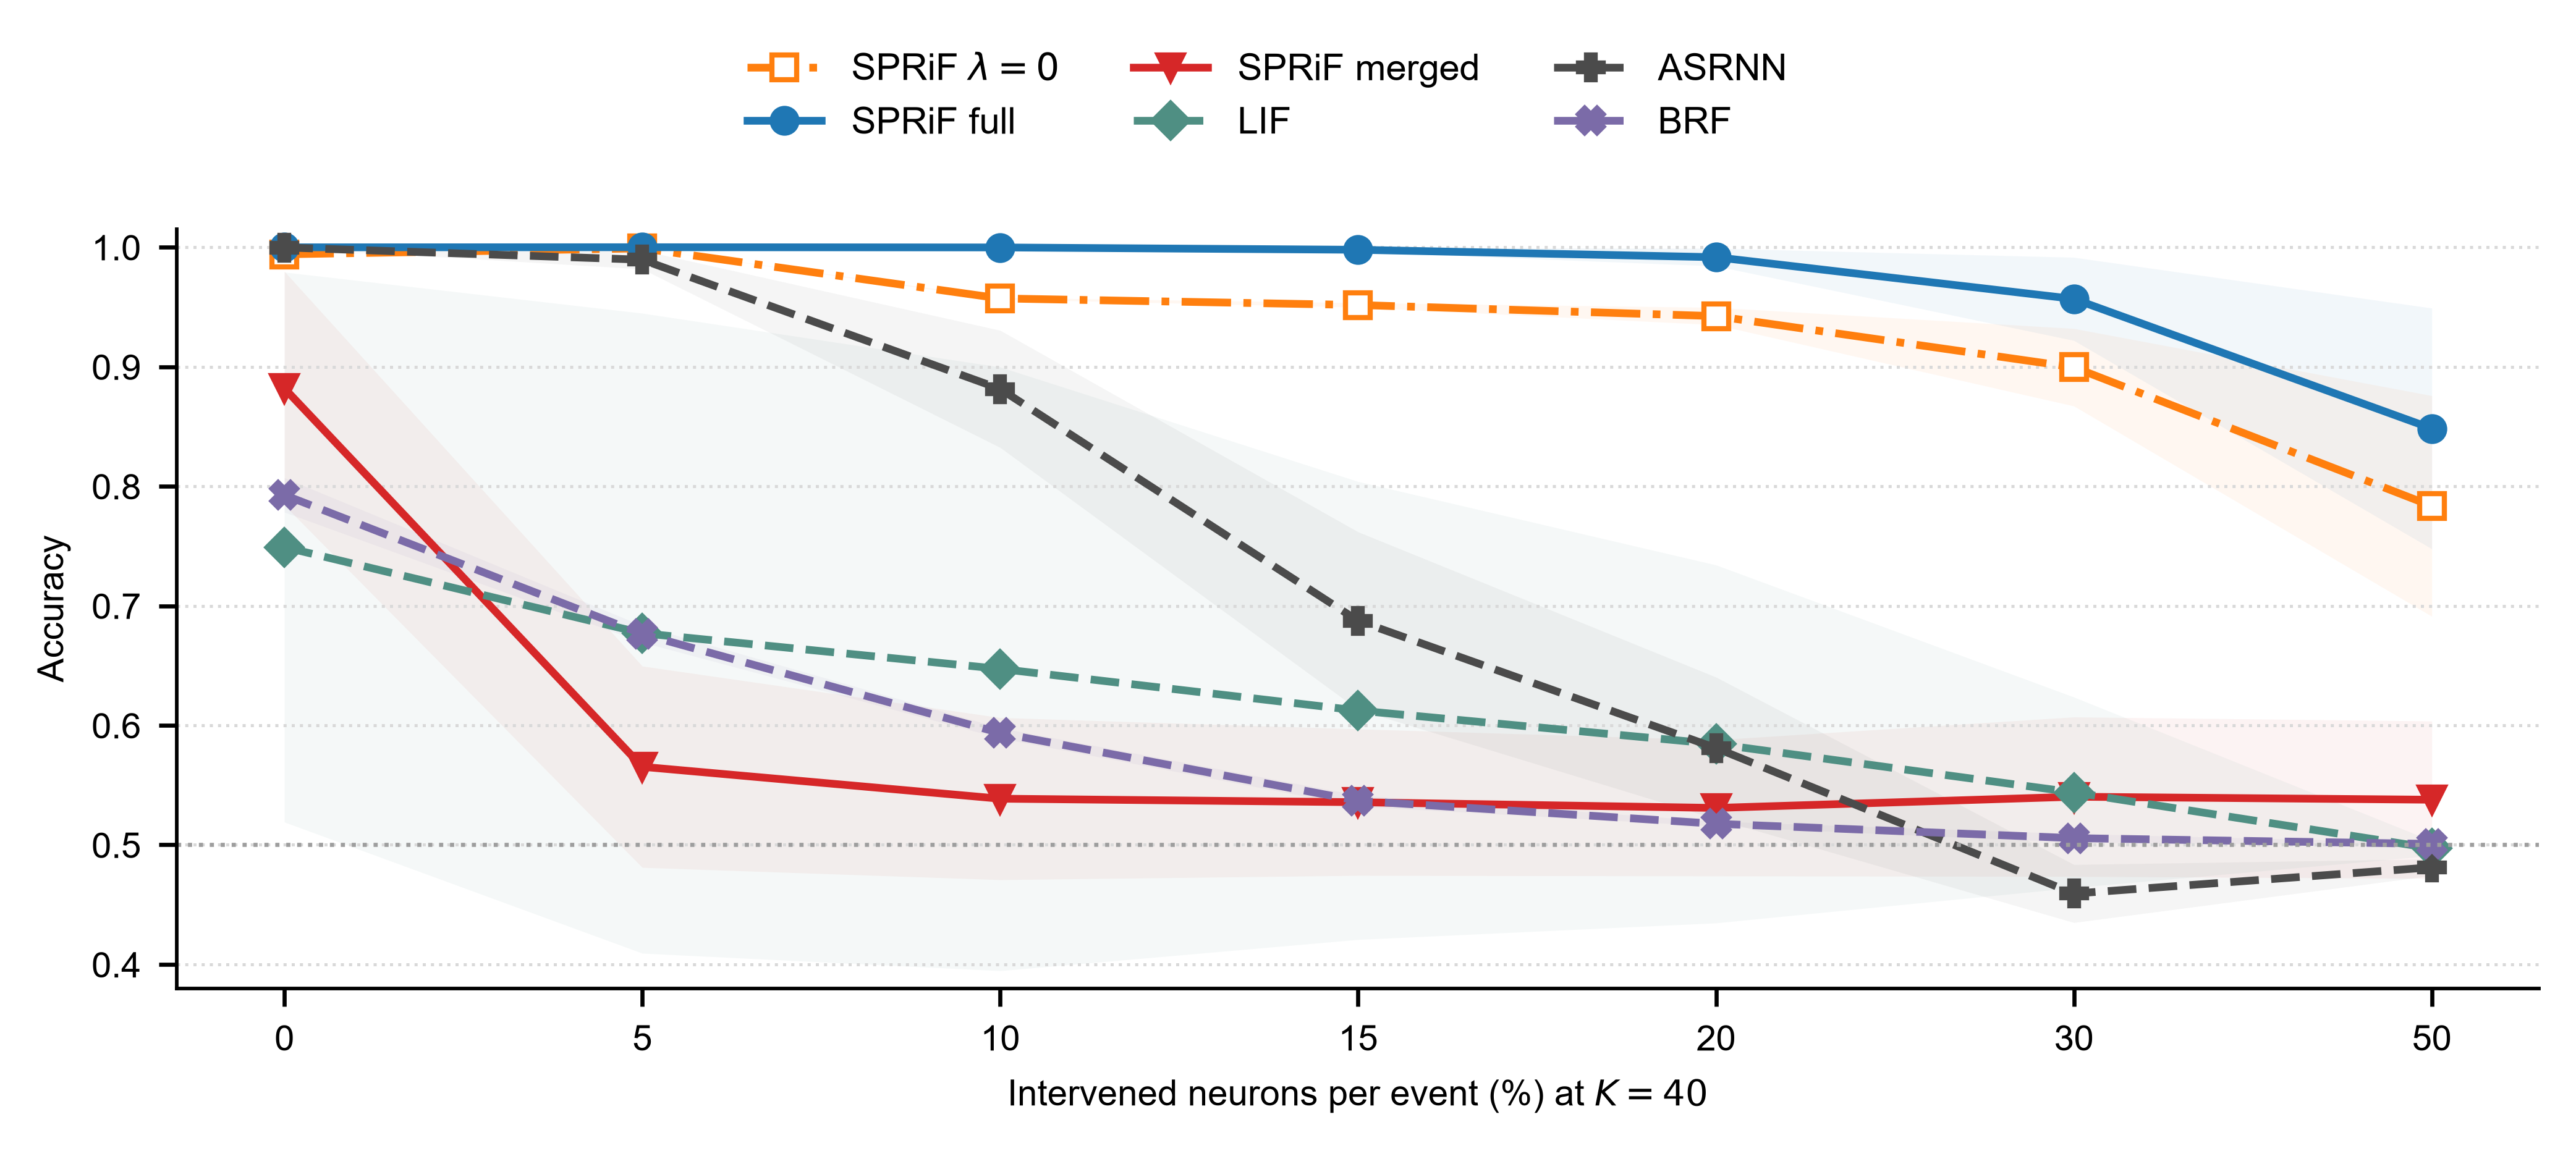
\includegraphics[width=0.94\textwidth]{figures/si_dms_fraction_response.png}
\caption{SI-DMS fraction response at the unseen intervention count $K=40$. Curves show means over three seeds after averaging each seed over five delays; shaded bands show seed standard deviations. The point at 0\% is the clean condition, and 15\% is the intervention fraction used during training.}
\label{fig:supp_sidms_fraction}
\end{figure*}

\subsection{Model Controls and Implementation Checks}
\label{supp:sec:sidms-integrity}

At an intervention timestep, the selected membrane coordinate is placed above threshold before spike computation. Under the hard threshold rule in Eq.~\eqref{eq:supp_spike}, this forces an actual spike, after which the model's ordinary reset rule is applied. The intervention follows the native threshold and reset path and ends with the model's standard update after a spike.

\begin{table*}[tbp]
\centering
\small
\setlength{\tabcolsep}{4pt}
\begin{tabular}{p{0.22\textwidth}p{0.33\textwidth}p{0.35\textwidth}}
\toprule
Implementation check & Specified behavior & Verification result \\
\midrule
Coverage & Each model/seed evaluates every configured combination of delay, $K$, and fraction. & All 18 runs contain 215 rows, giving 3,870 saved condition rows. \\
\midrule
Forced spike & Every selected unit emits a spike when $K>0$. & The saved evaluation metrics record a fraction of 1.0 for selected units that emitted spikes across all 3,780 rows with interventions. \\
\midrule
Shared controls & Model comparisons use the same probes. & Within a seed/delay/$K$/fraction condition, batches and intervention masks are shared across models. \\
\midrule
Reset path & Forced spikes trigger the same reset rule as ordinary spikes. & Interventions are applied before thresholding; the resulting spike triggers the standard reset update. \\
\midrule
Recurrent path & Forced spikes follow ordinary network communication. & The emitted spike is supplied to the learned recurrent pathway at the next timestep. \\
\midrule
SPRiF slow state & A forced spike leaves the slow spectral state unchanged at that timestep. & Eq.~\eqref{eq:supp_slow_insulation} gives $\Delta\mathbf{x}_t^{\mathrm{reset}}=\mathbf{0}$; recurrent communication enters the next timestep through $W_{\mathrm{rec}}\mathbf{z}_t$ when recurrence is present. \\
\bottomrule
\end{tabular}
\caption{Implementation checks for the SI-DMS intervention.}
\label{tab:supp_sidms_integrity}
\end{table*}

For SPRiF, let the reset direction be $\mathbf{r}=[1,\lambda_j]^\top$. The identity for resetting the fast state is
\begin{equation}
\mathbf{u}_t-\bigl(\widetilde{\mathbf{u}}_t-z_t\theta\mathbf{r}\bigr)=\mathbf{0},
\label{eq:supp_reset_residual}
\end{equation}
The slow state has no local reset update:
\begin{equation}
\Delta\mathbf{x}_t^{\mathrm{reset}}=\mathbf{0}.
\label{eq:supp_slow_insulation}
\end{equation}
These are structural identities of the stated update. They formalize the SI-DMS distinction: forced spikes alter the fast discharge state through actual spike and reset events, while the slow spectral state remains unchanged by local reset at that timestep.

\section{Formal SPRiF Specification and Analysis Protocols}
\label{supp:sec:dynamics}

\subsection{Slow Spectral State}
\label{supp:sec:slow-state}

The slow spectral state $\mathbf{x}_t\in\mathbb{R}^3$ evolves as
\begin{equation}
\mathbf{x}_t = A\mathbf{x}_{t-1} + B I_t,
\label{eq:supp_slow}
\end{equation}
where
\begin{equation}
A =
\begin{bmatrix}
\alpha & 0 & 0 \\
0 & \rho\cos\omega & -\rho\sin\omega \\
0 & \rho\sin\omega & \rho\cos\omega
\end{bmatrix}, \quad
B =
\begin{bmatrix}
1-\alpha \\
1-\rho \\
0
\end{bmatrix}.
\label{eq:supp_AB}
\end{equation}
The first coordinate is a real exponential trace,
\begin{equation}
x_t^0 = \alpha x_{t-1}^0 + (1-\alpha)I_t,
\label{eq:supp_real_mode}
\end{equation}
and the second and third coordinates form a damped rotational pair driven through the first oscillatory coordinate:
\begin{align}
x_t^1 &= \rho\cos\omega\, x_{t-1}^1 - \rho\sin\omega\, x_{t-1}^2 + (1-\rho)I_t, \\
x_t^2 &= \rho\sin\omega\, x_{t-1}^1 + \rho\cos\omega\, x_{t-1}^2.
\label{eq:supp_rot_mode}
\end{align}
The eigenvalues of $A$ are $\alpha$ and $\rho e^{\pm i\omega}$. We parameterize
\begin{equation}
\alpha=\sigma(\alpha_{\mathrm{raw}}),\quad
\rho=\sigma(\rho_{\mathrm{raw}}),\quad
\omega=\pi\sigma(\omega_{\mathrm{raw}}),
\label{eq:supp_param}
\end{equation}
so $\alpha,\rho\in(0,1)$ and $\omega\in(0,\pi)$, giving spectral radius $\max(\alpha,\rho)<1$. These sigmoid parameterizations keep the slow spectral state strictly stable for all finite values of the learned raw parameters.

\paragraph{Bounded-input stability.}
Let $q=\max(\alpha,\rho)<1$ and suppose $|I_t|\leq M$. Because the rotational block is $\rho R_\omega$, $\lVert A^k\rVert_2=q^k$. Unrolling Eq.~\eqref{eq:supp_slow} gives
\begin{equation}
\lVert\mathbf{x}_t\rVert_2
\leq q^{t+1}\lVert\mathbf{x}_{-1}\rVert_2
+\lVert B\rVert_2 M\frac{1-q^{t+1}}{1-q}.
\label{eq:supp_bibo_bound}
\end{equation}
Thus the influence of the initial state decays geometrically and every bounded input sequence produces a bounded slow state. This guarantee applies to the intrinsic slow transition; stability of the recurrent network is outside this bound.

Under a constant input $I_t=c$, the real mode converges to $c$. The rotational pair converges to the unique fixed point
\begin{align}
\mathbf{x}^{\mathrm{osc}}_\ast
&=
\bigl(I-\rho R_\omega\bigr)^{-1}
\begin{bmatrix}
(1-\rho)c \\
0
\end{bmatrix},
\label{eq:supp_osc_fixed_point}\\
R_\omega
&=
\begin{bmatrix}
\cos\omega & -\sin\omega \\
\sin\omega & \cos\omega
\end{bmatrix}.
\end{align}
Thus the first oscillatory coordinate generally differs from $c$ when $\omega\neq0$.

For a unit input impulse at $t=0$ with $\mathbf{x}_{-1}=\mathbf{0}$, the impulse response of the slow state isolates the two retention modes separately:
\begin{align}
x_k^0 &= (1-\alpha)\alpha^k, \\
x_k^1 &= (1-\rho)\rho^k\cos(k\omega), \\
x_k^2 &= (1-\rho)\rho^k\sin(k\omega),
\end{align}
for $k\geq0$. The real mode provides monotone retention, whereas the rotational pair provides damped phase dynamics.

\begin{figure*}[!t]
\centering
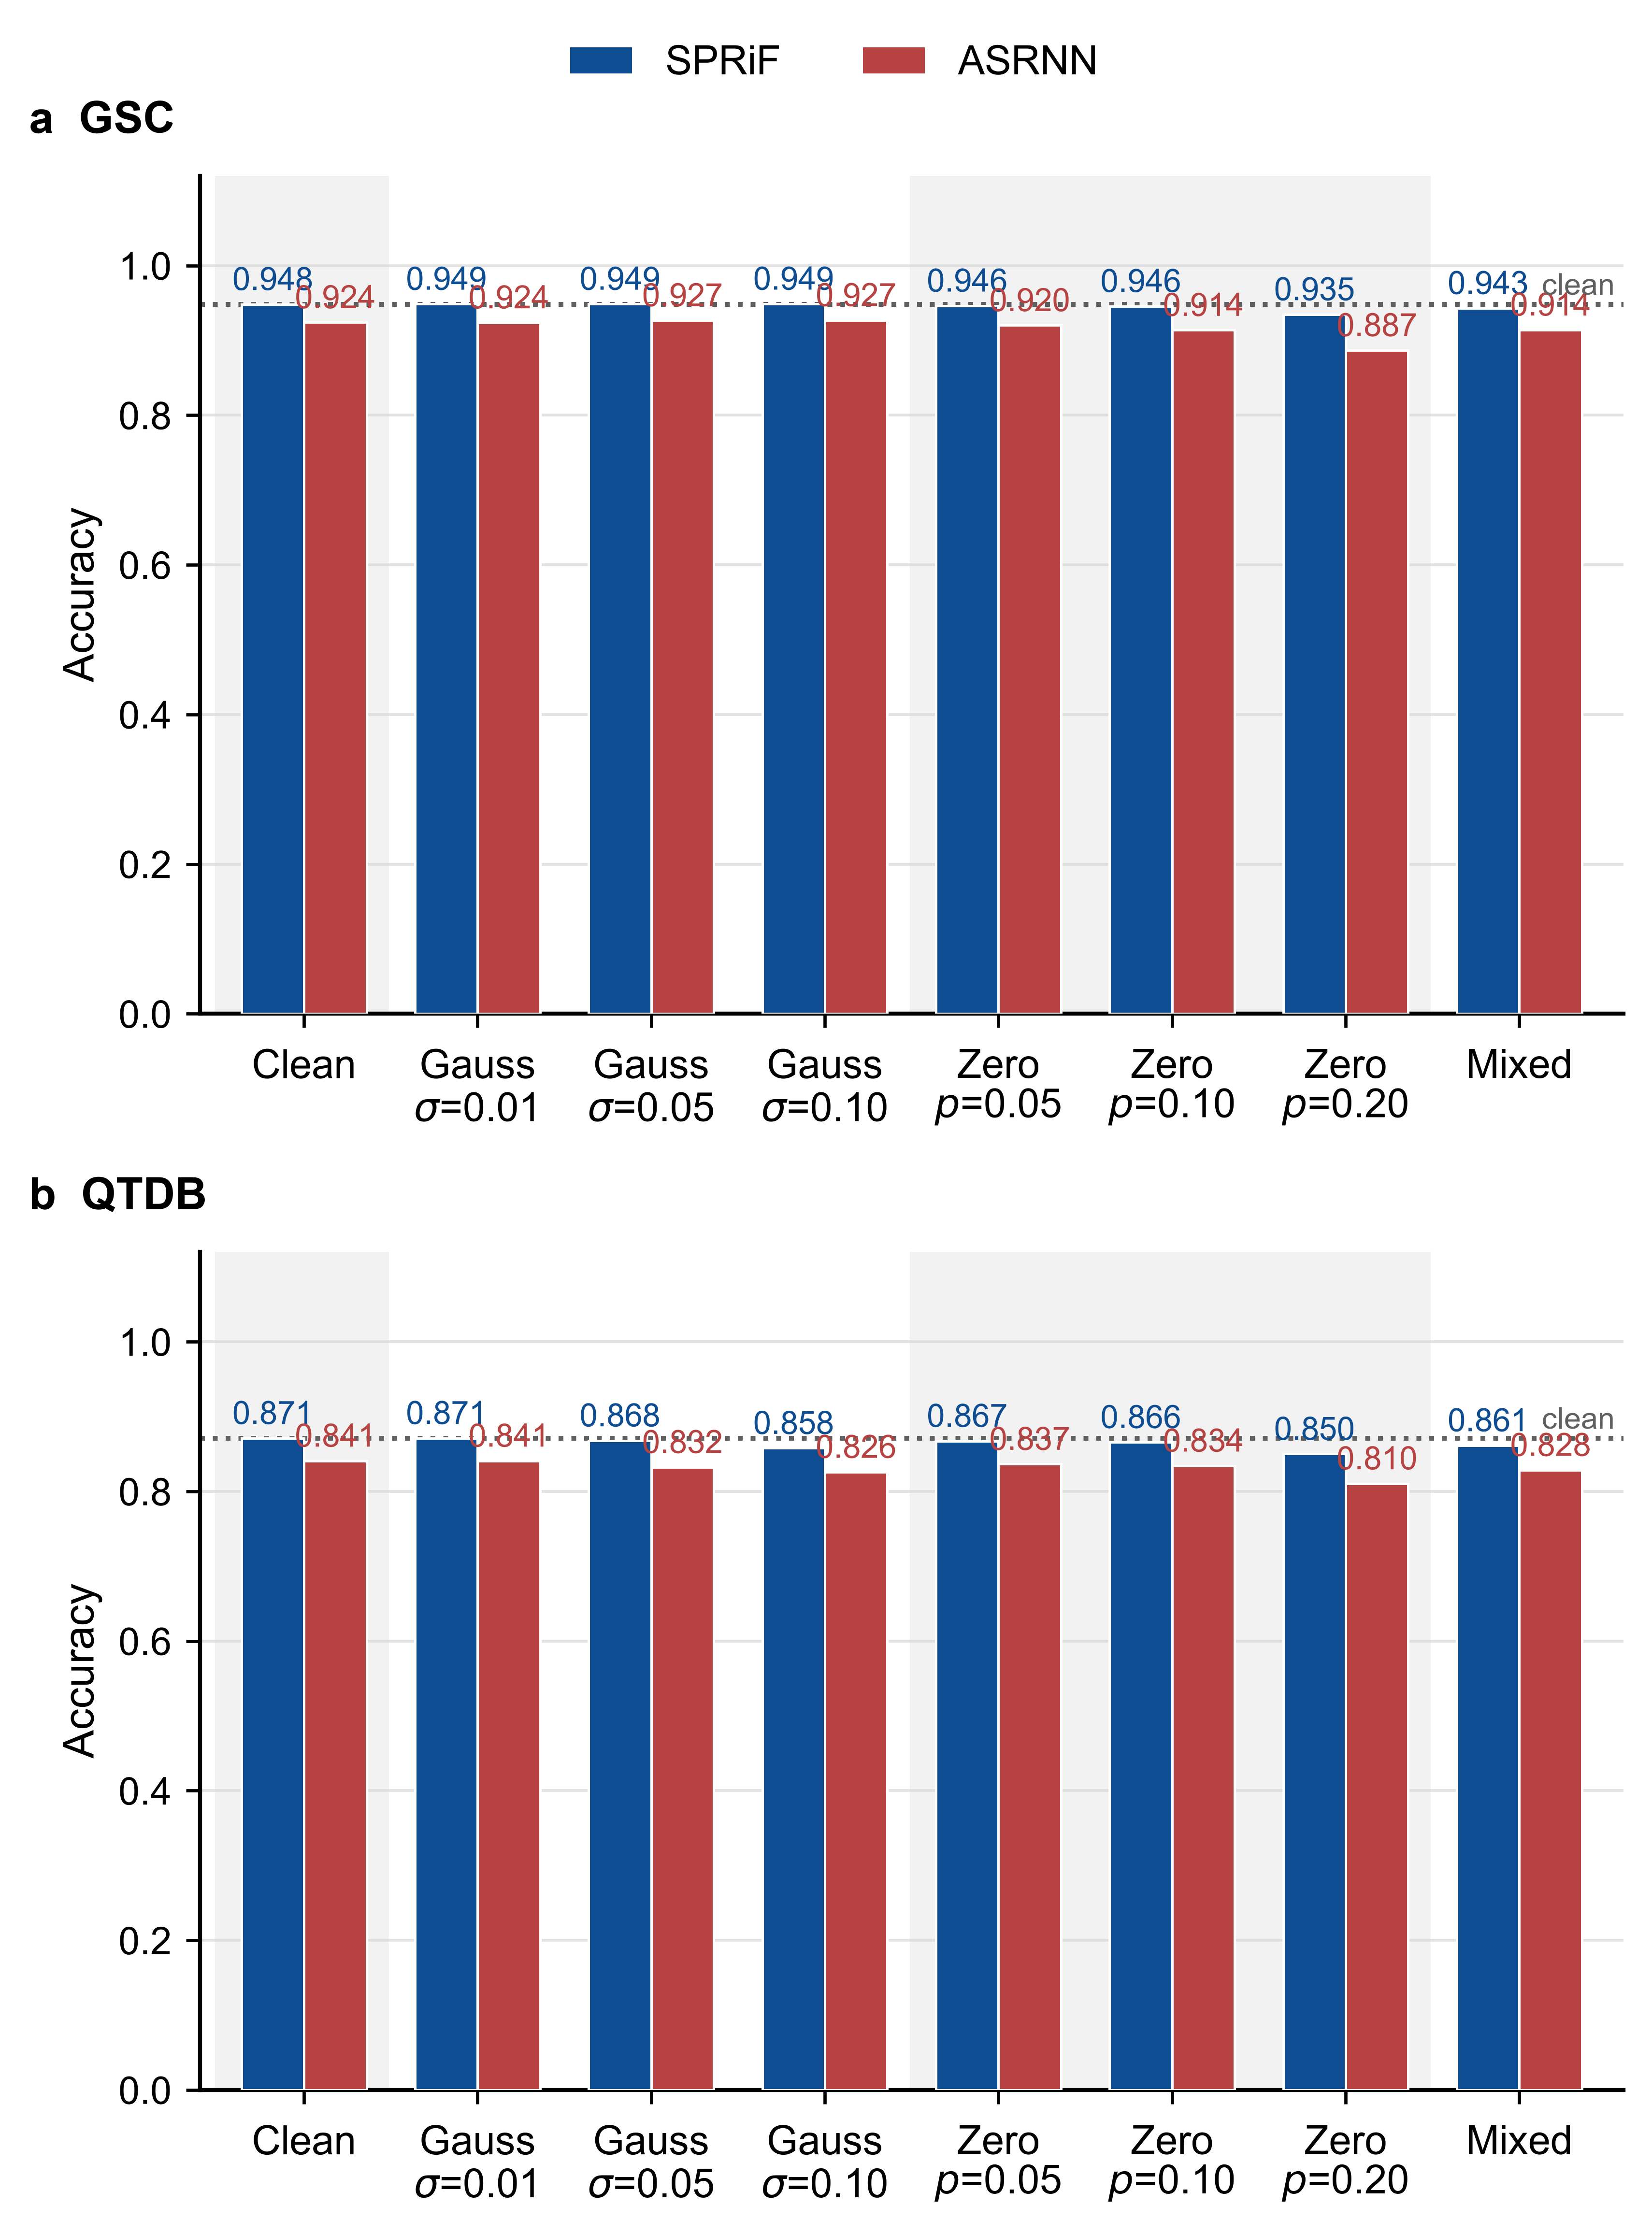
\includegraphics[width=0.59\textwidth]{figures/robustness_benchmark.png}
\caption{Perturbation diagnostic in feature space using saved checkpoints. SPRiF and ASRNN are evaluated on GSC and QTDB under additive Gaussian noise, random feature zeroing, and mixed perturbations. The clean values are those of the saved checkpoints used for the perturbation sweep; the main text reports separate benchmark summaries over five seeds.}
\label{fig:supp_robustness_diagnostic}
\end{figure*}

\subsection{Fast Discharge State and Projective Reset}
\label{supp:sec:fast-state}

The fast discharge state $\mathbf{u}_t\in\mathbb{R}^2$ receives a projection of the slow spectral state through $G\in\mathbb{R}^{2\times3}$:
\begin{align}
\widetilde{u}_t^0 &= \eta_0 u_{t-1}^0 + \kappa u_{t-1}^1 + (G\mathbf{x}_t)^0, \label{eq:supp_fast0} \\
\widetilde{u}_t^1 &= \eta_1 u_{t-1}^1 + (G\mathbf{x}_t)^1, \label{eq:supp_fast1}
\end{align}
with $\eta_0,\eta_1\in(0,1)$ parameterized as sigmoid-transformed raw variables. The membrane potential is $v_t=\widetilde{u}_t^0$, and the spike is
\begin{equation}
z_t = H(v_t-\theta),
\label{eq:supp_spike}
\end{equation}
where $H$ is the Heaviside step function.

Within each timestep, computation follows
\begin{align*}
I_t &= W_{\mathrm{in}}\mathbf{s}_t+W_{\mathrm{rec}}\mathbf{z}_{t-1}+b, \\
\mathbf{x}_t &= A\mathbf{x}_{t-1}+BI_t, \\
\widetilde{\mathbf{u}}_t &\to v_t=\widetilde{u}_t^0, \\
z_t &= H(v_t-\theta), \\
\mathbf{u}_t &= \widetilde{\mathbf{u}}_t-z_t\theta\mathbf{r}.
\end{align*}
This order matches the main text and confines the local reset update to the fast discharge state.

Component-wise, projective reset is
\begin{align}
u_t^0 &= \widetilde{u}_t^0 - z_t\theta, \\
u_t^1 &= \widetilde{u}_t^1 - z_t\theta\lambda_j.
\end{align}
Setting $\lambda_j=0$ recovers scalar subtraction on the membrane coordinate; a learned $\lambda_j$ allows reset to act along $[1,\lambda_j]^\top$ in the fast state.

\paragraph{Invariance under direct reset.}
Denote the slow and fast states immediately before local reset by $(\mathbf{x}_t^{-},\widetilde{\mathbf{u}}_t)$ and immediately after reset by $(\mathbf{x}_t^{+},\mathbf{u}_t)$. The update above gives
\begin{equation}
\mathbf{x}_t^{+}=\mathbf{x}_t^{-},\qquad
\mathbf{u}_t=\widetilde{\mathbf{u}}_t-z_t\theta[1,\lambda_j]^\top.
\label{eq:supp_direct_reset_invariance}
\end{equation}
Therefore the direct reset residual of the slow state is exactly zero for either spike outcome. This guarantee concerns the current timestep; in a recurrent layer, $z_t$ can affect $I_{t+1}$ through the ordinary learned recurrent pathway.

\subsection{Surrogate Gradient}
\label{supp:sec:surrogate}

The forward pass uses the hard threshold in Eq.~\eqref{eq:supp_spike}. During backpropagation, the threshold derivative is replaced by the multi-Gaussian surrogate~\cite{asrnn}:
\begin{equation}
\begin{aligned}
\frac{\partial z_t}{\partial v_t} \approx \gamma\big[&
a_0 \mathcal{N}(v_t-\theta;\,0,\sigma_0^2) \\
&{}-a_1\mathcal{N}(v_t-\theta;\,\mu_1,\sigma_1^2) \\
&{}-a_1\mathcal{N}(v_t-\theta;\,-\mu_1,\sigma_1^2)\big],
\end{aligned}
\label{eq:supp_surrogate}
\end{equation}
where $\sigma_0=0.5$, $a_0=1.15$, $\mu_1=0.5$, $\sigma_1=3.0$, $a_1=0.15$, and $\gamma=0.5$. The forward dynamics remain unchanged.

\subsection{Initialization, State Size, and Cost}
\label{supp:sec:initialization-cost}

The initialization ranges for each task are listed in Table~\ref{tab:supp_arch}. For each decay $q\in\{\alpha,\rho,\eta_0,\eta_1\}$, a time constant $\tau_q$ in steps is mapped to $q=\exp(-1/\tau_q)$ before conversion to its unconstrained raw parameter. Raw variables are initialized so that the transformed $\alpha$, $\rho$, $\eta_i$, and $\omega$ values fall in the listed ranges; after initialization, optimization proceeds in the unconstrained raw parameter space.

Each SPRiF neuron stores five state values $(x^0,x^1,x^2,u^0,u^1)$ and has 13 dynamics parameters per neuron: $\alpha_{\mathrm{raw}}$, $\rho_{\mathrm{raw}}$, $\omega_{\mathrm{raw}}$, $\eta_{0,\mathrm{raw}}$, $\eta_{1,\mathrm{raw}}$, $\kappa$, the six entries of $G\in\mathbb{R}^{2\times3}$, and $\lambda$. The weight matrices $W_{\mathrm{in}}$ and $W_{\mathrm{rec}}$ and the bias $b$ follow the layer architecture.

For a layer of width $h$, the local state update cost is $O(h)$ because each neuron uses slow and fast states of fixed size. When recurrent connectivity is enabled, the $O(h^2)$ multiplication $W_{\mathrm{rec}}\mathbf{z}_{t-1}$ dominates for both recurrent SNNs based on LIF neurons and SPRiF layers.

\subsection{Analysis Protocols}
\label{supp:sec:analysis-protocols}

For the impulse response and temporal kernel analyses in the main text, we inject a unit impulse into trained SPRiF neurons and record 100 steps of intrinsic evolution of the slow state with zero subsequent input. The four displayed SPRiF trajectories use the 10th, 40th, 70th, and 90th percentiles of learned $\alpha$. Under this protocol, the response shapes reflect the learned spectral parameters, with direct local reset confined to the fast state.

For the GSC and QTDB panels that compare models, the SPRiF real mode at the 90th percentile is paired with the available trained ASRNN membrane kernel having the closest derived $\tau_m$. Each displayed kernel is normalized by its peak magnitude, and spectra from the real coordinate are aggregated across neurons.

The analysis of learned reset directions uses the $\lambda$ values shown in the mechanism figure of the main text. Across QTDB, GSC, and PS-MNIST, the reported $\lambda$ distributions span both signs, and the figure reports weak Pearson correlations with firing rate, $\alpha$, and $\omega$ ($|r|\leq0.191$). These observations support diverse projective reset directions in the fast discharge state. The sign of $\lambda$ is interpreted here through its computational reset geometry, without a universal biological interpretation.

\subsection{Feature Perturbation Diagnostic}
\label{supp:sec:perturbation-diagnostic}

Figure~\ref{fig:supp_robustness_diagnostic} reports a perturbation diagnostic in feature space on GSC and QTDB using fixed checkpoints. Controlled input corruptions are widely used to probe non-adversarial robustness~\cite{hendrycks2019benchmarking}, while additive Gaussian jittering is a standard perturbation of amplitude for time-series inputs~\cite{iwana2021empirical}. Motivated by these evaluation practices, we apply additive Gaussian noise, random feature zeroing, and their combination to saved SPRiF and ASRNN checkpoints, with matched perturbation settings within each condition. The diagnostic records responses under the specified perturbations. The benchmark table, summarized over five seeds, remains the basis for comparison with published results.

\bibliography{sprif2027}

\end{document}
